\documentclass[swedish,a4paper,11pt]{article}
\usepackage{fullpage}
\usepackage{babel}
\usepackage[utf8]{inputenc}
%\usepackage[T1]{fontenc}
%\usepackage[british,swedish]{babel}


\usepackage{amsmath}
\usepackage{amssymb}
\usepackage{amsthm}
\usepackage{color}
\usepackage{float}
\usepackage{listings}
\usepackage{fontenc}
\usepackage[hidelinks]{hyperref}
\usepackage{graphicx}
\usepackage{float}
\usepackage[export]{adjustbox}
\usepackage{wrapfig}
\usepackage{tabularx}
\usepackage[table,xcdraw]{xcolor}
\usepackage{array}
\usepackage{enumitem}
\usepackage[section]{placeins}

\usepackage{multirow}
\usepackage{caption}
\captionsetup[table]{name=Tabell}
\captionsetup[figure]{name=Figur}



\begin{document}
\begin{titlepage}
\title{\textbf{Analys och utvärdering av användbarhet 
SF Bio, SF.se \\
    Människa och Datorinteraktion 5Hp \\ Uppsala University -- Spring 2015 \\
    Grupp O
      }}

\author{
Oliver Campeau, Mikael Sernheim, Sam Rönnlund, Josef Svensson, Philip Åkerfeldt \\
\textup{Dept. of Information Technology}\\
\textup{Uppsala University}\\
\textup{Uppsala Sweden}\\
}
\date{\today}

\end{titlepage}

\maketitle

\begin{figure}[hb]
\centering

\includegraphics[scale=1]{SFBioLogo.png} 
\end{figure}

\newpage
\tableofcontents 

											
\hfill \break
\break										
\textbf{Vår prototyp} \hfill \textbf{\href{http://user.it.uu.se/~mise2899/home.html}{Prototyp}}
\pagebreak


\section{Introduktion}

Vi har fått i uppgift att analysera SF bios hemsida (hädanefter refererad till som SF.se) utifrån perspektivet människa-datorinteraktion. SF.se är en plattform som främst är till för att förse SF:s kunder med en biljett-bokningstjänst och att marknadsföra sitt filmutbud. Sidan tillhandahåller även information och tjänster för sin medlemsklubb “bioklubben” samt en del filmnyheter. 
 
\subsection{Systemets sammanhang} 
SF.se är huvudsakligen till för att tillhandahålla SF:s kundbas med biljettbokning online. Innan systemets sattes i bruk skedde fjärrbokning endast per telefon så det har underlättats markant genom möjligheten med Internetbokning. Fördelarna med bokning online är många för både SF samt dess kunder, till exempel att det inte behövs en kommunikation mellan kund och en säljare i person för att bokning ska vara möjlig vilket kan vara en fördel för båda parter.

\subsection{Användargrupp} 
De som använder tjänsten är de som har tillgång till Internet och som planerar ett eventuellt biobesök. SF.se hade under 2012 ungefär 1 550 000 besökare i månaden och förköpsbiljetter inhandlade på Internet under året motsvarade 67.3\% av den totala försäljningen. Under året hade SF ungefär 12 miljoner besökare detta resulterar i att tjänsten har använts till att boka ca 8 miljoner\footnote{SF Bio, 2012  \\
\url{http://www.sf.se/om-sf-bio/sf-bios-verksamhet/}\\ (Hämtad 2015-02-05)} biljetter. Enligt Statistiska centralbyrån\footnote{ Statistiska Centralbyrån, 2013\\ \url{http://www.scb.se/Statistik/_Publikationer/LE0108_2013A01_BR_IT01BR1401.pdf} \\ (Hämtad 2015-02-05)} så använde under 2012 närmare 95\% av alla personer mellan 16-74 år Internet så vi kan inte säga särskilt mycket om vilken ålderskategori som använder hemsidan utan det kan var alla olika åldrar som använder tjänsten.

\subsection{Analysavgränsning}
Denna rapport är mestadels centrerad kring biljett-bokningssystemet på SF:s hemsida. Vi valde att fokusera på detta för att vi tror att det är den primära anledningen till att användare besöker hemsidan. Analysen rör även SF.se i sin helhet då vi bedömer att hemsidans helhet också påverkar hur biljett-bokningssystemet upplevs. Med vår avgränsning menar vi processen från att användaren landar på startsidan tills hen står på sidan som bekräftar ett köp/reservation. Det handlar alltså om att välja var, när och vad kunden vill se, samt att betala eller reservera dessa platser, för att till sist få en bekräftelse på detta.

\newpage
\section{Metod}
Vi valde att kombinera intervjuer med en enkät. Varje gruppmedlem fick välja ut en person som de intervjuade om deras uppfattning om hemsidan och sedan ombads personen som intervjuades att göra en bokning och uttrycka sina åsikter om själva bokningstjänsten. Under intervjun användes metoden Think Aloud, det vill säga att person i fråga använder sig av hemsidan och berättar vad de gör och vad de tänker när de det. I intervjuerna gav vi dem instruktioner såsom att de skulle beställa biljetter för en viss film, salong och datum. Vi fick idéen om att använda Think Aloud av vår föreläsare Thomas Lind\footnote{Lind, Thomas; doktorand Uppsala universitet\\
\url{http://katalog.uu.se/empinfo/?languageId=1&id=N10-1507}}, och läste sedan en artikel\footnote{Nielsen Norman Group. 2012 \url{http://www.nngroup.com/articles/thinking-aloud-the-1-usability-tool/}\\{(Hämtad 20
5-02-05)}} av Jakob Nilsen som också talar om ämnet.

Enkäten gjordes i Google Forms och spreds sedan via Facebook till vår användargrupp. Vi valde att ha ganska övergripande frågor med möjlighet att ge extra feedback för att vi ville att så många som möjligt skulle ha tid med att göra undersökningen. De första frågorna i enkäten behandlar väldigt kort användarnas demografi, för att se om de fanns stora skillnader mellan kön eller åldrar. Därefter ställs frågor angående användandet av systemet och positiva/negativa saker med det. Enkäten är med som bilaga.

\subsection{Användare} 
De personer som vi har med i vår undersökning var av olika åldrar, kön och erfarenhet av hemsidan. Efter vi hade gjort enkäten så delade alla fem personer i analysgruppen den på sin Facebook-sida och alla som hade besökt SF.se någon gång fick vara med och svara. Vi fick därför över 260 svar på enkäten och det var ganska jämnt fördelat mellan män och kvinnor, det var överlägset mest personer i åldern 15-29 år som svarade vilket vi antar beror på att vi alla har flest vänner på Facebook i den åldersgruppen och det är också personer i den åldersgruppen som är mest aktiva på sociala medier.\\ De flesta av våra enkätdeltagare (över 80\%) hade använt sig av sidan mer än 4 gånger per år och dryga 40\% besökte den mer än 8 gånger per år. De fyra personerna som vi valde att intervjua var antingen personer som vi kände väl eller personer som hade någon speciell bakgrund eller färdighet som kändes relevant för att göra rapporten mer robust och intressant.\\
Två av personerna som intervjuades har någon slags bakgrund inom grafisk behandling alt. formgivning och dessa hade liten till mycket liten erfarenhet av hemsidan sen tidigare.\\
De två resterande personerna som intervjuades var "normala" användare, utan någon speciell bakgrund, och de hade ganska bra till bra erfarenhet av hemsidan sen tidigare.

\subsection{Undersökningsmiljö} 
Enkäten gjordes via Internet där vi inte hade någon kontroll över miljön för användarna. Intervjuerna utfördes på lite olika sätt och i olika miljöer. Tre intervjuer skedde öga-mot-öga där den intervjuade fick sitta med sin egen dator i sin hemmiljö utan tidsbegränsning och fick utföra en biljettbeställning. Två intervjuer skedde över videosamtal genom Skype där den intervjuade satt med sin dator hemma hos sig och skärmen delades för intervjuaren att se. 

\newpage
\section{Resultat}

Efter att ha analyserat svaren på enkäten så kan det konstateras att den generella åsikten om SF.se är positiv. Av våra drygt 260 bidrag så gav 84\% av de frågade betyget 3 eller mer (skala 1-5) på frågan om helhetsintrycket av hemsidan. Detta har att göra med att den anses fylla sitt syfte och dess design faller in i majoritetens smak. Den fullständiga enkäten finns som en klickbar länk i vår innehållsförteckning eller \href{https://docs.google.com/forms/d/1KFDziZeg0wwAXTIV-LeV9eBy-Oa-SH1aR7GebkXLKKI/viewform?c=0&w=1}{\textit{här}} och sammanställda resultat återfinns längst ner i dokumentet som tårtdiagram.\\

\noindent
\begin{wrapfigure}{r}{0.52\textwidth}
  \begin{centering}
    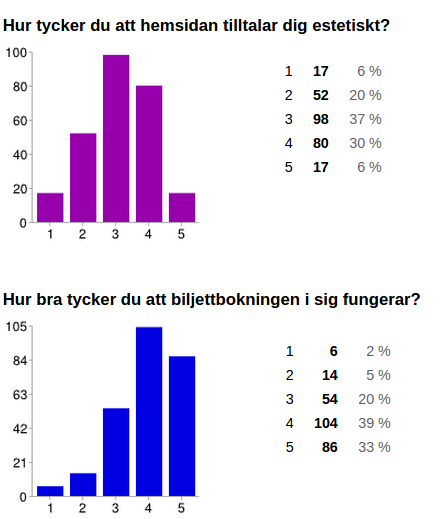
\includegraphics[width=0.48\textwidth]{charts.png}\\
  \end{centering}
  \caption{Tabeller från bifogad enkät}
\end{wrapfigure}

När vi går in på djupet på biljettbokning som är vårt huvudfokus pekar svaren på att funktionaliteten är bra med undantag från smådetaljer. På frågan hur bra biljettbokningen fungerar satte 69\% av deltagarna betyget 4 eller 5 (skala 1-5, där 5 är bäst).\\

Av de alternativ som gavs till våra enkätdeltagare om bra respektive dåliga beståndsdelar med SF.se så har vi fått fram följande. Genom tolkning av fritexten som deltagarna skrivit är det flera som angett att valet av stad är komplicerat och dåligt fungerande och i alternativen som gavs inkluderas det i “Hur man väljer biograf”. I vårt fritextalternativ fick vi även in flera bidrag som uttryckte missnöjda över att sidan inte alls var mobilanpassad.\\
\begin{center}
\begin{table}[h]
    \begin{tabularx}{0.9\textwidth}{|X|X|}
    \hline
    \rowcolor[HTML]{32CB00}
    Bra                                      & \cellcolor[HTML]{FF0000} Dåligt  \\[2ex] \hline
    Hur man väljer sittplats i salongen 79\% & Hur man väljer biograf 53\% \\[2ex] \hline
    Betalningssätt och säkerhetskänsla  57\% & Hur man väljer film 36 \%   \\[2ex] \hline
    \end{tabularx}
\caption{Data sammanställt från enkät}
\end{table}
\end{center}

Resultaten från våra intervjuer styrker utfallet från enkäten och gav oss detaljer på förbättring. Vi hade totalt 4 intervjuer varav två av dem valde att vara anonym resterande är angivna vid källor. 
Vid en intervju med Marcus Nystrand\footnote{Marcus Nystrand; Grafisk student på Beckmans Designhögskola. \\
2015, intervju den 4 Februari} belyste han vissa bristningspunkter och han uttryckte sig på följande sätt för att beskriva dessa: “För det första är sidan väldigt plottrig och det krävs för många klick för att komma till sin önskade destination. Man märker direkt att startsidan är spretig rent fokusmässigt. Man vet inte vart man ska lägga fokus och inte heller vart det är meningen att fokuset ska placeras. Utseendet på hemsidan är ganska välgjord om man bortser från vissa grafiska missar som är nybörjarmisstag för att vara helt ärlig. Filterfunktionen skulle behöva slipas lite på för den är ganska kass för tillfället.”

Åsa-Sara Sernheim\footnote{Sernheim, Åsa-Sara; magister i bildterapi, konstnär och formgivare.\\ 
2015, intervju den 4 Februari} påpekade några designdetaljer; “Headern är väldigt liten och de har valt ett typsnitt som är gjort för att vara mörkt mot ljus bakgrund, när de gör tvärtom så flyter det ihop och läsbarheten försämras.” Hon lade även till “För att vara Sveriges ledande biografer så känns hemsidan omodern. De borde jobba mer för att ge besökaren biografstämning. Just nu är det bara filmduken i bakgrunden som överhuvudtaget gör en ansats till det.”

I annan intervju med en kvinna i tjugoårsåldern som önskade att vara anonym så kom åsikter om när man väljer en film/föreställning: “När man har tryckt att man ska välja en film så borde det vara en stor bild på denna film i mitten av skärmen, inte en liten bild högst uppe till höger som man knappt kan se!” sedan tillade hon “det är också väldigt liten text som gör det svårt att läsa.”

\subsection{Användarsyfte} 
Vi hade ingen fråga i vår enkät som handlade om varför våra deltagare använde sig av hemsidan. Däremot frågade vi i alla våra intervjuer och där fick vi veta att främst av allt ville deltagarna boka biljett och samtidigt var det populärt att se hur utbudet av filmer såg ut. 

\subsection{Användarkontext} 
Systemet som analyserats har ett ganska smalt användningsområde.  Situationerna då systemet i fråga används är inte jättemånga. De vanligaste anledningarna som dök upp under intervjuerna var; att boka/köpa biljetter; planera inför ett kommande biobesök; eller att kolla upp information om filmer eller inför ett kommande biobesök. 

\newpage
\section{Diskussion}
Vi är i grunden nöjda med vårt val av undersökningar. Enkäten gav en bred bild av hur den stora publiken tyckte om hemsidan och våra intervjuer gav en djupare bild av hur en mindre skara tyckte. Vi trodde från början att användarna primärt använde systemet för att boka biljetter och valde därför att inte fråga varför de använde systemet i enkäten. Men när vi genomfört intervjuerna visade det sig att folk använde sidan till annat än biljettbokning så insåg vi att det kan ha varit ett misstag att ej ta upp den frågan i enkäten, vi känner dock att vi fick ett bra och konsekventa svar på den frågan genom intervjuerna.\\ 
Valet av metoden Think Aloud tycker vi var ett bra val, det kändes som om att man fick en naturlig bild av vad användarna tyckte om systemet. Samtidigt kunde man styra intervjun i vilket håll man ville utan att det kändes hackigt. Vi känner att vi fick ut mer värdefull data av intervjuerna och gärna hade haft några fler för att få mer djupgående data från fler personer. Det för att få en ännu mer korrekt bild av vad användarna tycker om systemet och hur de använder det.

\subsection{Funktionsmässiga problem}
Efter en empirisk studie kunde några slutsatser dras och dessa grundades av åsikter från flera deltagare i studien. Några av dessa problem som belystes av deltagarna var bland annat antalet klick man behövde från att man kom in på sidan tills dess att man kunde genomföra sitt köp. 
Studien visade även att de användare som hade som mål att söka inspiration för ett framtida biobesök hade problem med att använda sig av hemsidans filtertjänst. Det fanns visserligen filter på hur man kunde sortera dom filmerna som visades men dessa var otydliga och hjälpte inte lika mycket som de borde ha gjort. 
En annan punkt som lyftes fram av flera intervjudeltagare var att det på samma del av hemsidan fanns en “topplista” som lika bra kunde ha varit en filterfunktion. Den hade fyllt sin funktion lika bra, om inte bättre, som ett filter i den redan existerande filtermekaniken. 

\subsection{Utseendemässigt} 
Det första man möts av på SF.se är en, i proportion till resten av hemsidan, stor reklambild. Ovanför den är ett litet avsnitt där man kan välja stad, biograf och film och en huvudmeny. Den inledande reklamen är så stor att den täcker upp största delen av skärmen och skapar en förvirrande sida. Detta är speciellt ett problem på datorer med lite lägre upplösning på skärmen, då dessa annonser är något som tar upp hela sidan. Ett annat problem som kan härledas till den stora annonsen är att om den inte laddas in  så hamnar merparten av en ruta för att välja vilken stad man är i under webbläsarmenyn, vilket kan vara en anledning till att många klagar på att man alltid glömmer att byta stad. Det kan uppstå om t.ex.användaren använder ett plug-in för att blockera annonser, man går in via mobiltelefonen, att det är driftstopp på deras annonsserver eller liknande.

\noindent

\begin{figure}[H]
\centering
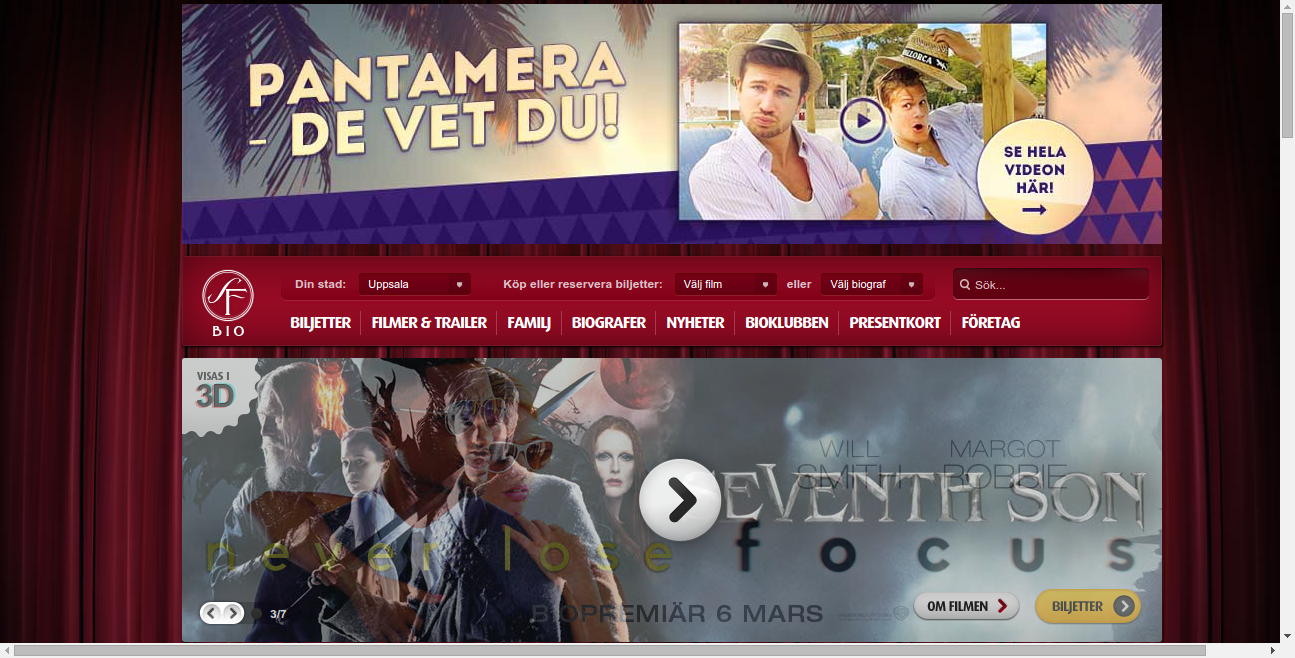
\includegraphics[scale=0.27]{StartsidaLow.png} 
\caption{Befintlig startsida med låg upplösning}
\end{figure}
									%% BILD PÅ STARTSIDAN OCH REKLAMEN %%

\subsection{Mindre användbarhets problem} 
Vi tyckte att det var intressant att flera personer i vår enkät noterade att SF.se inte alls var mobilanpassad på ett bra sätt. I enkäten fanns det ett allmänt missnöje kring huruvida den mobila versionen av hemsidan samt företagets app fungerade. I enkäten nämndes det även att om man använder sig av hemsidan en eller två gånger per år så vill man kanske inte ladda ner en app för att göra detta och man vill inte heller komma till en relativt dåligt utformad mobil version av hemsidan. Dessa saker känns som ganska enkla saker att fixa tycker vi.

\subsection{Stora användbarhets problem} 
Vi drar slutsatsen att våra intervjudeltagare i allmänhet anser att hemsidan för SF är väldigt rörig, plottrig och användare beskriver det som jobbigt att hitta rätt. Det finns för många knappar, för många val och användarvänligheten måste definitivt höjas. För många är SF.se enbart ett verktyg för att boka ett biobesök på och mer fokus bör läggas vid just den funktionen. Deltagarna efterlyser ett snabbare, enklare och mer tydligt sätt att boka sin vistelse på. Idag läggs ofta stor vikt på enkelhet, ‘less is more’, något SF.se bör ta lärdom utav. 

\subsection{Positiv återkoppling}
En mycket positiv och omtyckt funktion är själva platsbokningen i biosalongen. Användare kan enkelt välja antal sittplatser och få en tydlig översikt över vilka platser som är lediga/upptagna. Denna metod att välja sittplatser i biosalongen valde $\frac{3}{4}$ av våra deltagare som en positiv sak på hemsidan.

\newpage


\section{Designimplikationer}
Som beskrivet i resultatet så var det val av film och stad som användarna hade störst problem med. Många av användarna ville att valet av stad skulle ske automatiskt. Eftersom valet av stad var en liten rullgardinsmeny var detta något som användaren ofta missade. Hade de gjort valet av film innan de bytte stad fick det göras om när de valde rätt stad. Därför valdes detta som förstaprioritet vid en nydesign. \\
I vår undersökning var det självklart för användarna vilken stad de ville gå på bio i, därför när systemet inte såg det som lika självklart skapade det irritation. Samtidigt om man vill använda hemsidan för att kolla på trailers och se vilka filmer som går på bio är inte detta något problem, eventuella pop-ups eller att man är tvungen att välja vilken stad innan man kan göra något annat kommer även det att skapa irritation hos de användarna. Generellt skulle man kunna säga att om systemet kan göra ett bra antagande av vad användaren vill till exempel vilken stad man vill gå på bio i, kommer hen att uppskatta det när det blir rätt, blir det fel så är problemet lika stort som om systemet inte gjorde något antagande. \\
Med tanke på avgränsningarna som antogs angående systemets primära användningsområden påverkades designen på så sätt att den blev väldigt fokuserad kring en smidig bokningsprocess eller en lätt navigering menade för framtida filmbesökare. Detta betyder rent designmässigt att mycket har skalats ner eller tagits bort helt medan andra delar har framhävts eller förstorats för att göra navigering enklare och göra besöket på hemsidan mer intuitivt. Vid en nydesign vill vi att det ska vara svårare att göra fel, men när användaren ändå gör fel ska de inte behöva straffas för det och behöva börja om från början. Ett mål är att det ska vara intuitivt och följa ett mönster så att användaren känner igen sig i de olika stegen, om man förstår hur det fungerar i första steget ska man även förstå de nästkommande stegen. Detta uppnås genom att olika uppgifter som användaren behöver utföra kommer byggas upp ackumulativt vilket gör det lättare att förstå vad som kräver fokus, men det kommer även lämna möjlighet att till exempel ändra vilken film man ska se på.\\
Om användaren inte gör något fel under sin bokning kommer det ta ungefär lika lång tid som på det gamla systemet, dock kommer färre fel att begås eftersom vissa val kommer vara mer synliga och obligatoriska att göra. Men om ett fel görs kommer hen att snabbare vara tillbaka i rätt del i bokningen och inte behöva göra om flera steg som redan gjorts. Sammantaget kommer tiden för alla användningar av systemet att sjunka eftersom användarna kommer begå mindre fel och när de begår felen kommer det inte att skicka tillbaka dem till början. 

\newpage
\section{Designteorier}
Har förklaras varför vi valde våra designteorier och vad vi tycker att dem tillför.

\subsection{Mentala representationer} 
Mentala representationer är ett begrepp inom kognitionsvetenskapen som beskriver en inre bild av yttre händelser, i detta fall hur användaren tycker och tänker om systemet i fråga\footnote{Nielsen Norman Group, 2010 \\ \url{http://www.nngroup.com/articles/mental-models/}\\ (Hämtad 2015-02-27)}. Den mentala representationen som vi tänker att användaren först tänker ut vilken film de ska se, sedan kollar de vilken dag och tid som de kan se denna film och sist var i salongen man vill sitta och hur man vill betala. Detta är svårt att förutspå hur alla användare skulle föredra att använda sig av bokningssystemet men vi anser att detta är en korrekt bild av hur folk gillar att använda sig av sidan. Det känns mest vanligt att kunder till SF.se känner att de vill se en specifik film snarare än att tänka att man vill se bio en viss tid en dag, oavsett vilken film det är.

\subsection{Perception} 
I vårt resultat kom vi fram till att många ansåg första sidan som rörig och plottrig. Alldeles för mycket information gjorde det svårt att navigera på sidan och gjorde processen att boka ett biobesök betydligt svårare än den behöver vara. Vår hjärna är flexibel men har även begränsningar när det kommer till att kunna uppfatta information. Hade vi försökt ta in allt som finns på SFs startsida samtidigt hade vi drunknat i information. Därför måste vi vara selektiva i våra val av vad vi ska ta till oss vid en särskilt tidpunkt (TH6).

På gamla sidan fanns det alldeles för många alternativ, t.ex. välja stad, filmaffischer och en gigantisk banner/filmaffisch som byter film den visar efter ett par sekunder efter ett rullande schema. Alla dessa alternativ kunde eventuellt leda till biljettbokningssystemet. För någon, som enbart är ute efter att boka en biljett, kan detta givetvis uppfattas som ett stort störningsmoment, något vårt resultat även visat. Därför kommer vi i vår nya design av SFs hemsida gruppera informationen så att en potentiell biljettbokare ska kunna hitta den informationen fort och slippa behöva ta till sig reklam och processera detta innan den uppfattar var biljettbokningen kan göras. Vi ska även vara mer konkreta och inte upprepa all information lika mycket som sidan gör idag utan skapa ett enkelt användargränssnitt.   

\subsection{Mönsterigenkänning} 
En viktigt del i vår nya design av SFs hemsida är att vi vill ändra saker så att det blir bättre men samtidigt inte ändra på för mycket av designen så användare inte ska känna igen sig. Vi vet från vår undersökning och analys att en majoritet av användarna tyckte att hemsidan var från medelbra till bra. Vår enkät visade också att ungefär 80\% av användargruppen besökte sidan fler än tre gånger per år. Detta går att läsa i resultatet på enkäten som är bifogat. Vi tänker då att det finns en stor chans att besökaren redan är bekant med sidan och därför är det viktigt att vi inte ändrar för mycket så användaren inte känner igen sig. Människor är otroligt duktiga på att känna igen mönster och känner sig mer hemma bland något de känner igen(TH2). Man vill gärna känna igen mönster, så mycket att man till och med gör det ibland när det inte finns ett mönster där. Vi tyckte därför att det är en otroligt viktig aspekt att ta hänsyn till när vi gör vår nya design av hemsidan. 

\subsection{Kunskap och kännedom}
En viktig del vi kommer fokusera på i den nya designen av SFs hemsida är att göra det så lätt som möjligt att boka biljett. Vi vill skapa en automatisk process så att användaren behöver tänka så lite som möjligt vid biljettbokning. Med detta menar vi att vi inte vill skapa en sida som introducerar nya saker för användaren, utan mer fokuserar på enkelhet och saker som användaren kan känna igen sig i. Allt för att skapa en process som går fort och där användaren inte behöver lära sig nya saker för att kunna boka en biljett. (TH6)

\subsection{Affordans och gestaltningslagar} 
Engelskans affordance är ett svårt begrepp att översätta till svenska och vi anser att affordans är en tillräckligt bra översättning så att folk förstår vad vi menar. Affordans är en ekologisk teori (TH6), något vi anser att mannen som själv uppfann begreppet bäst kan beskriva. Detta är ett utdrag från hans bok The Ecological Approach to Visual Perception(1979); ”The affordances of the environment are what it offers the animal, what it provides or furnishes, either for good or ill.“

Vi har även försökt implementera gestaltningslagar i form av Figure-Ground när det gäller våra tryckbara knappar. Detta stycke av gestalts psykologi handlar om hur olika objekt står sig mot varandra, hur vi uppfattar vissa figurer baserat på vad det är för objekt som är i närheten. I vårt fall handlar det om att försöka göra en knapp att visuellt verka “tryckbar”, att den ska stå ut ifrån sin bakgrund och likna en knapp i verkliga livet.\footnote{Michael Tuck\\ \url{http://sixrevisions.com/web_design/gestalt-principles-applied-in-design/}\\ (Hämtad 2015-02-27)}

 I vår nya design av SFs hemsida har vi skapat en miljö med affordans, vi har en knapp på framsidan där det står “Köp biljetter” och när man för musen över den så reagerar den genom att ändra färg. Vi har även designat knapparna på ett sätt som får dem att stå ut ur bakgrunden. Detta har vi gjort genom att göra dem rundade i kanterna och med lite mörkare toner mot kanterna som liknar skuggor.

\newpage
\section{Vår nya design} 
Det första vi gjorde var att ta bort den stora reklamen som låg högst upp på sidan. Detta gjorde vi eftersom den helt enkelt tog upp för mycket skärmyta, speciellt vid låg upplösning. Vi har istället valt att flytta ner all form av reklam så den ligger under vår meny. Den enda reklamen som är kvar är filmreklamen som låg under menyn. Reklamen har dock gjorts mindre eftersom personerna i vår undersökning tyckte att den var för stor i relation med hur mycket information den gav.
\noindent

\begin{figure}[H]
\centering
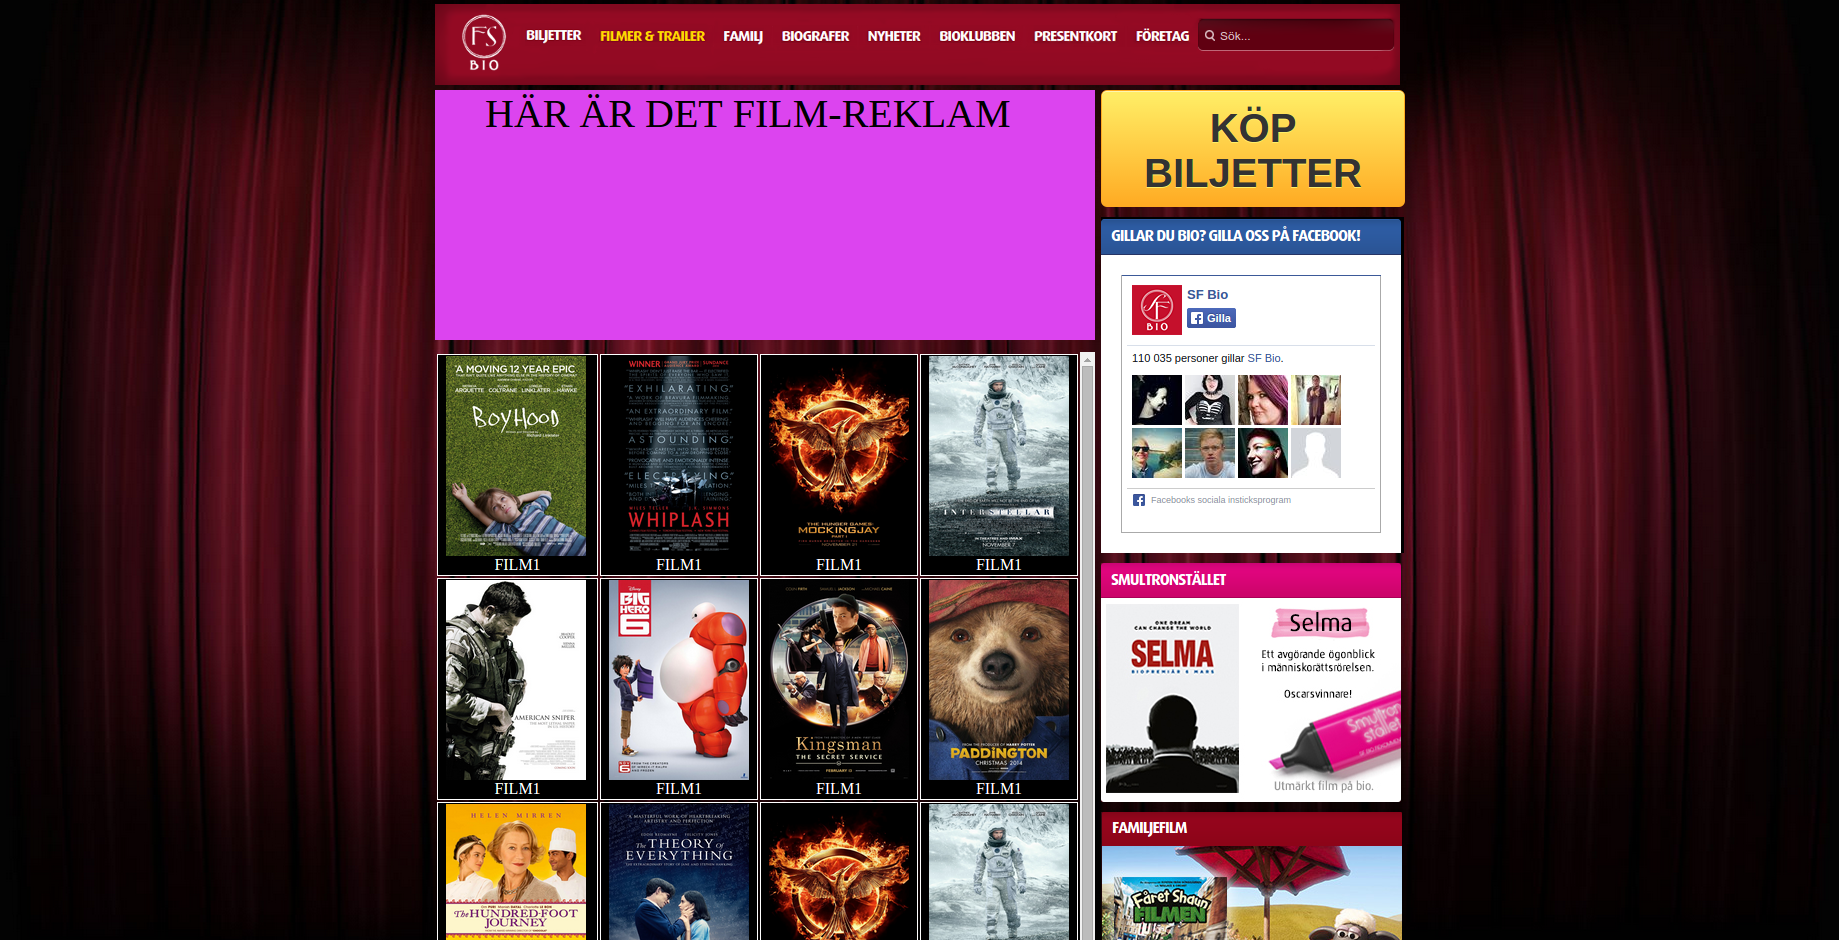
\includegraphics[scale=0.20]{ourdesign.png} 
\caption{Sidan efter vår nya design}
\end{figure}


								%% Sidan efter omdesign %%

Menyn överst på sidan försvinner när man scrollar ner för att ge mer skärmyta till vårt innehåll, men så fort man scrollar upp dyker den upp så att man ska kunna navigera lätt på sidan och se vilken sida man nu är inne på. Från menyn har vi tagit bort valet att välja stad och att snabbvälja vilken film man vill se eller vilken biograf man vill kolla på. Valet av stad sker automatiskt och om det inte fungerar att välja automatiskt kommer en dialogruta när man klickar på knappen “Köp biljetter”. Detta var en funktion som väldigt många av användarna bad om att få eftersom många av dem glömde att välja stad och fick sedan börja om med sin bokning. Valet att ta bort stad och biograf gjordes eftersom den innan krävde 4 klick för att komma till val av föreställning, vilket även vår nya bokningssystem gör. Därför känns det redundant när det inte sparar klick och tid utan bara skapar förvirring för användarna när man kan göra samma sak på flera olika sätt. Istället lades en knapp som heter "köp biljetter" till för dem som vill boka biljetter snabbt. 
\noindent

\begin{figure}[H]
\centering
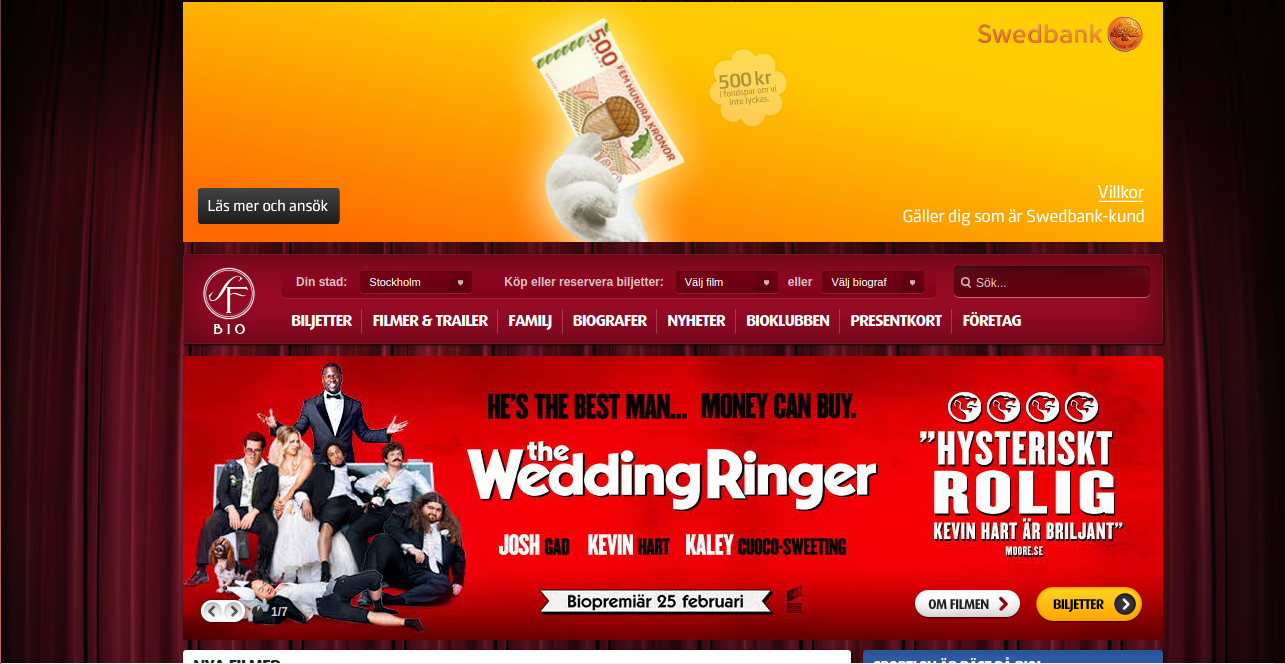
\includegraphics[scale=0.27]{befintligstartsida.png} 
\caption{Startsida innan vår nya design}
\end{figure}


%% Startsidan innan vår omdesign %%



I våra intervjuer sa användarna att de använde sidan till att boka biljetter och att kolla vilka filmer som gick på bio. Vi valde därför att lägga mest fokus på det på startsidan. Under filmreklamen la vi ett rutnät av filmposters samt namnet på filmen under postern för att det ska vara så tydligt och synligt som möjligt för användaren att se vilka filmer som går. Här tog vi även hänsyn till om personen har sett postern innan vilket gör det lättare att hitta till den filmen. Om man ställer muspekaren på någon av filmerna läggs en mörkare ton på bilden så att användaren förstår att det finns något man kan göra med bilden. Det kommer även upp två knappar över bilden, den ena för att få se information och den andra för att boka biljetter till en visning av filmen. Vi valde att ha båda möjligheterna för att ge de två grupperna av användare det som de ville använda hemsidan till.
\\

\newpage
När användaren trycker på den nya knappen “Köp biljetter” kommer användaren slussas vidare till en ny sida där hen möts av en dialog där användaren först måste välja stad innan någon annan handling kan genomföras. Detta förutsatt att den automatiska lokaliseringen inte fungerade. Detta gjorde vi för att se till att användaren inte glömmer att välja stad vilket leder till att användaren måste göra om biljettbeställningen från början. Faktumet att användare glömde välja stad var något som SF:s nuvarande hemsida led utav.  

\noindent

\begin{figure}[h]
\centering
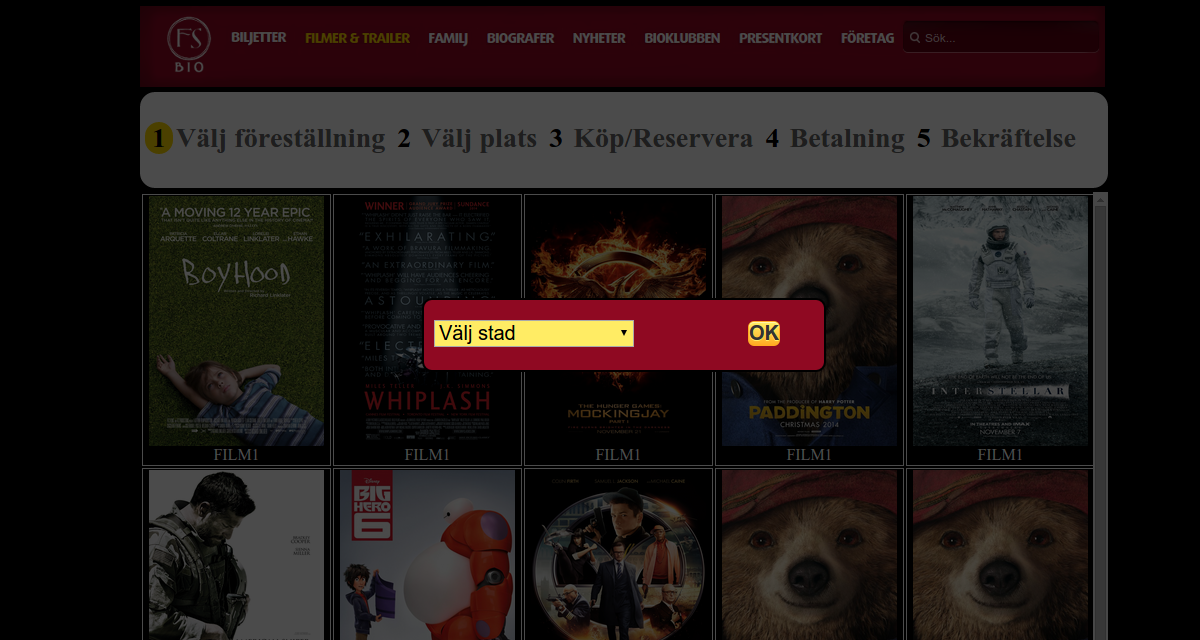
\includegraphics[scale=0.27]{valavstad.png} 
\caption{Meny för att välja stad}
\end{figure}

%% VÄLJ STAD BILDEN %%
\newpage
Sidan som användaren slussas till ser nästan exakt ut som startsidan med den största skillnaden att antalet filmer som finns på varje rad har ökat. Vi designade sidan på just det speciella sättet för att användaren skulle fokusera på filmerna som kan väljas och inget annat. 
Högst upp på sidan finns en statusrad som beskriver vilket steg i biljettbeställningen användaren befinner sig i. Steget som användaren befinner sig i framhävs med en urskiljande färg. Statusfält kan användas för att navigera sig till tidigare steg i beställningen om det skulle vara något som hen önskar att ändra.\\

\begin{figure}[H]
\centering
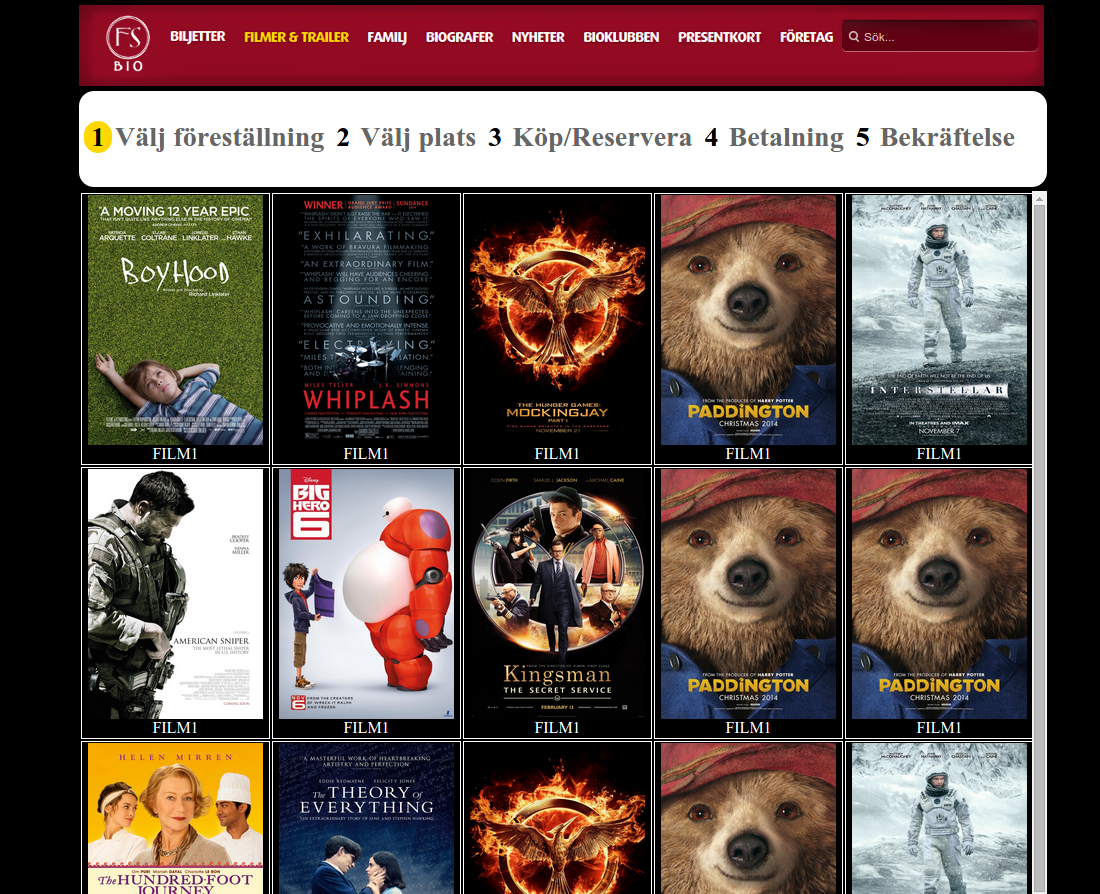
\includegraphics[scale=0.27]{filmermeny.png} 
\caption{Ny design för menyn av valbara filmer}
\end{figure}

%% BILD PÅ FILM MENY %%

\newpage
När valet av film har gjorts visas detta i ett nytt fält som glider ner mellan statusraden och rutnätet med valbara filmer. I det nya fältet visas en stor ikon av den valda filmen för att minimera förvirring. Bredvid bilden för vald film finns en beskrivning av filmen samt en rullgardins-meny där användaren kan välja vilken dag hen vill se föreställningen. 

\begin{figure}[H]
\centering
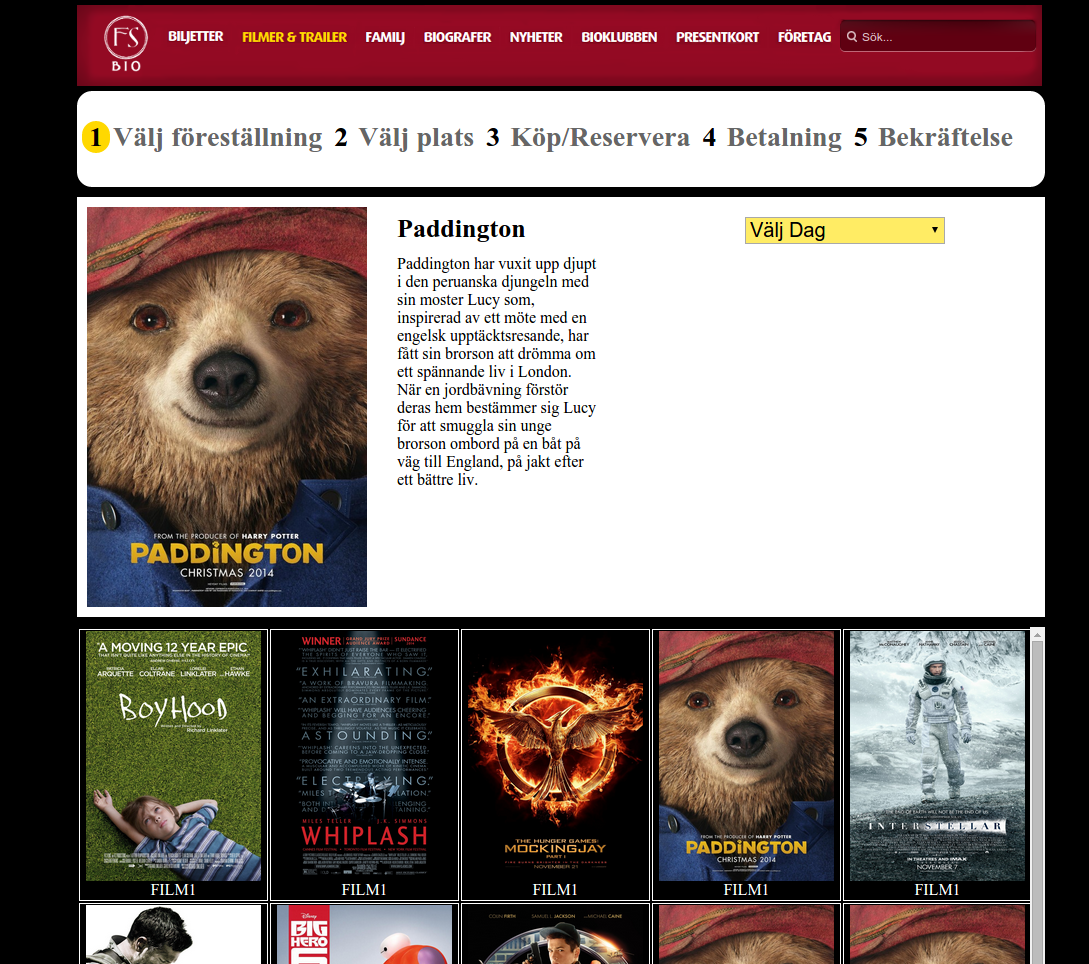
\includegraphics[scale=0.27]{valdfilm.png} 
\caption{Ny design för menyn vid vald film}
\end{figure}
%% BILD PÅ VALD FILM %%

\newpage
När användaren har valt dag kommer det upp en lista med vilka biografer och vilken salong som visar föreställningen samt information tillhörande varje föreställning. Informationen som listas är: tid för föreställning, antal platser kvar, version (talat språk, om filmen är textad eller ej). Förutom information finns det, för varje föreställning, en knapp som ger användaren alternativet att gå vidare för att köpa eller reservera biljetter till föreställningen.  

\begin{figure}[H]
\centering
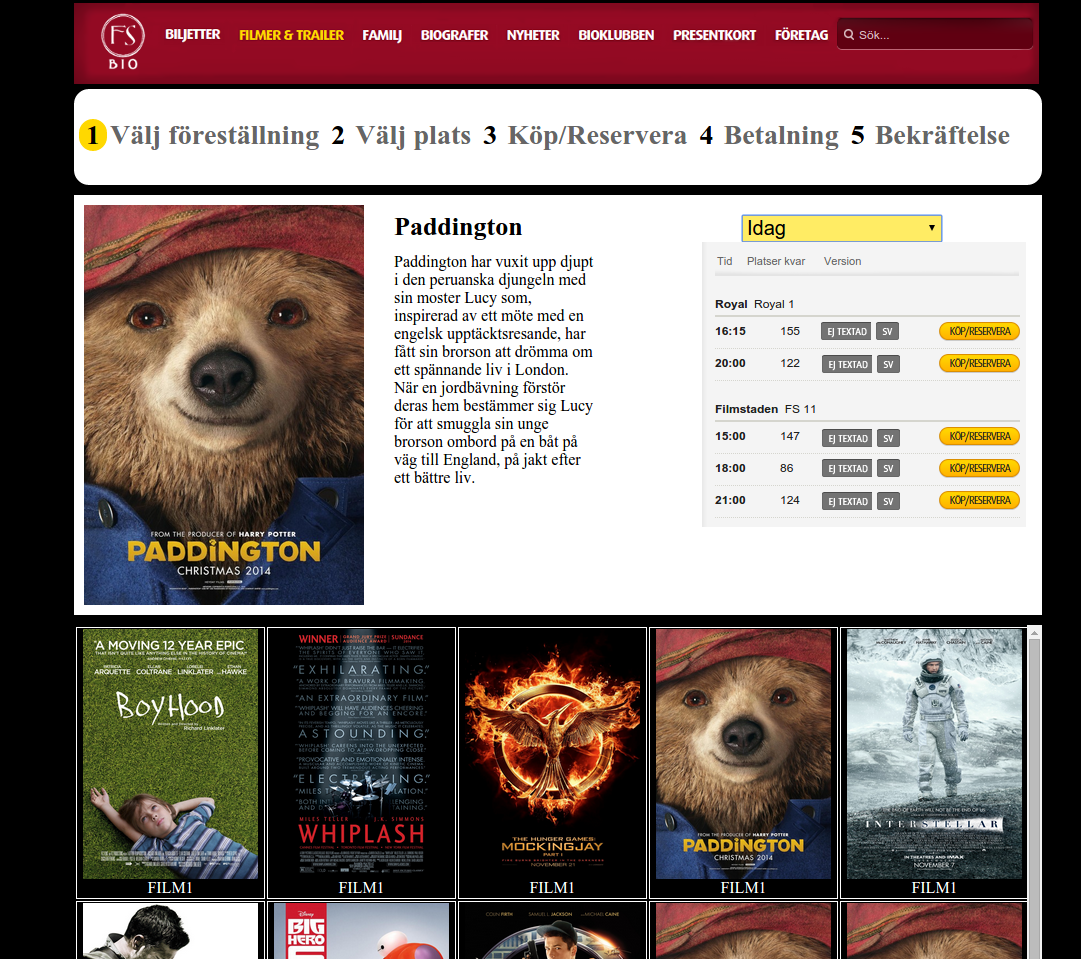
\includegraphics[scale=0.27]{valddag.png} 
\caption{Ny design för menyn vid vald film samt dag}
\end{figure}


%% BILD PÅ VALD DAG %%

\newpage

Efter man har tryckt på köp/reservera från föregående “Välj föreställning”-steget så kommer man till denna bild ovan BILDNUMMER. Sättet man väljer platser på är ganska lik nuvarande som finns på SF.se. Enda skillnaden är att vi har en stor bild på filmen så att det är väldigt liten risk att man köper en biljett till fel film. På SFs orginalsida är det en mindre bild än den som vi använder. Det är tänkt att man väljer sina platser som man alltid har gjort och sedan trycker på “Gå vidare”-knappen. En funktion som finns i vår implementation men inte i SFs är att om man står i steg 2 “välj plats” så går det att klicka på det föregående steget uppe i headern och då går man till det steget. Det är alltså enkelt att koordinera sig genom ett köp.

Våra övriga steg “Köp/Reservera”, “ Betalning” och “Bekräftelse” tänker vi att det ska se exakt ut som på SFs hemsida. Detta handlar om hur man betalar och vi känner att det är ett bra, beprövat och säkert sätt att göra ett köp på Internet. Det är inget som vi skulle vilja ändra.
\begin{figure}[H]
\centering
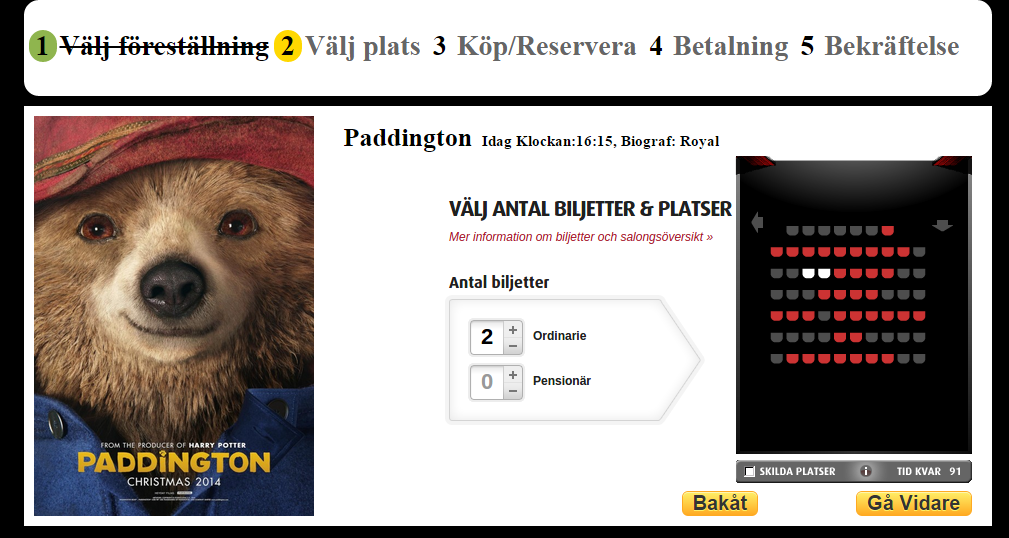
\includegraphics[scale=0.27]{valdplats.png} 
\caption{Ny design för menyn när man ska välja plats}
\end{figure}

\newpage
\section{Alternativa design} 
Vi hade flera idéer innan vi valde den som presenterades ovanför. En av de delarna som diskuterades mest i gruppen var huruvida vi skulle använda oss av bilder och ett namn under så som vår nya design ser ut nu eller om vi skulle ha en version som mer liknande den nuvarande SF hemsidan med en lista där alla filmtitlar står. Den befintliga layouten som SF använder ser ut som figuren nedan. 

\begin{figure}[H]
\centering
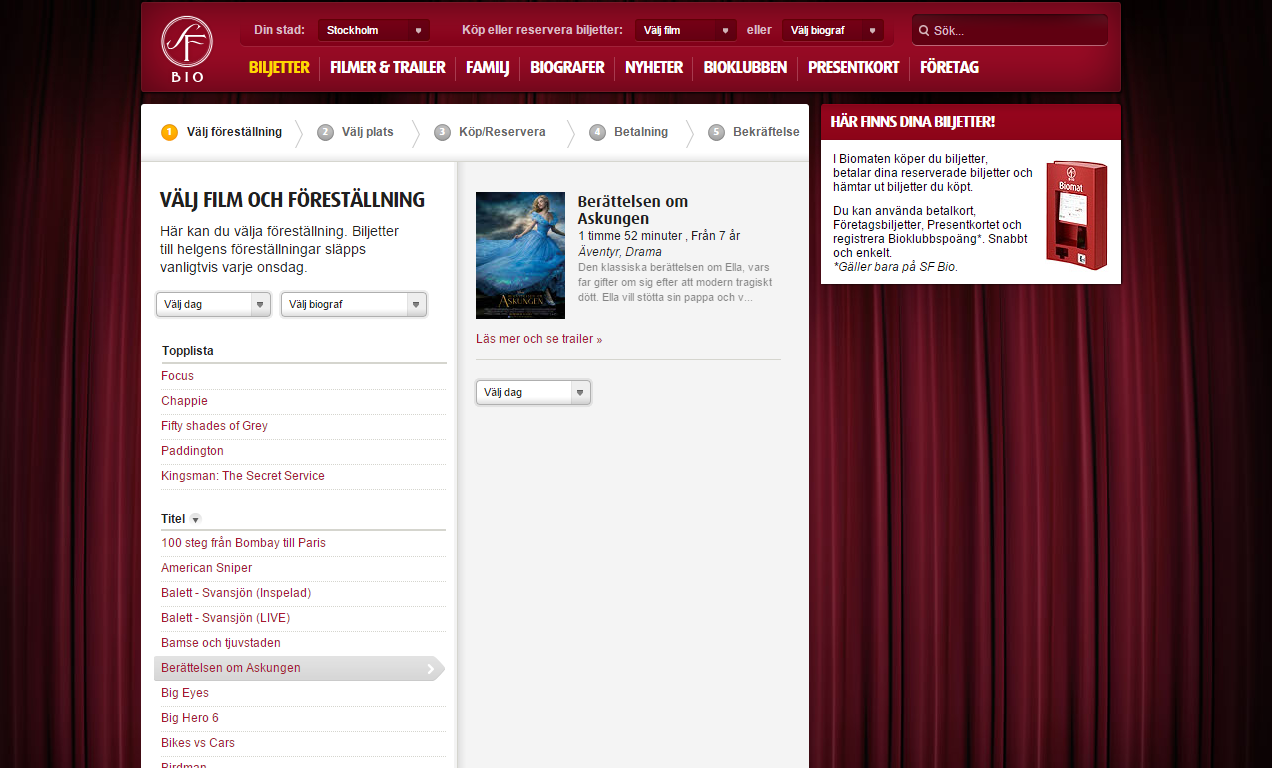
\includegraphics[scale=0.45]{LISTVY.png} 
\caption{Nuvarande layout för SF:s "Välj film och föreställning"}
\end{figure}

Med skillnaden att bilderna och texten på höger sida ska vara större. Vi valde tillslut bort den designen eftersom vi tänkte att det är bättre att läsa namnet och att få se framsidan på den. Sedan ska man få mer information om den om man klickar på den som vår design var tänkt att göra. Vi föredrog denna design eftersom att det finns nog användare som inte känner igen namnet på en film men kanske har sett reklam för den massvis med gånger och då hjälper bilden väldigt mycket. Sedan finns det användare som inte bestämt vilken film de vill se och då kan bilder från filmen hjälpa till att skaffa ett intresse, det är ju bara bättre om man kan se filmerna före man har klickat på någonting.

En annan sak som vi diskuterade och som vi fick påpekat i en av våra expert evaluations var tiden under platsbokningen som syns i figur 10 och om den skulle vara kvar eller ej. Vi ansåg att den skulle vara kvar då vi tänker oss att om den skulle försvinna så tror vi att det skulle skapa stor förvirring för användaren om sidan helt plötsligt uppdaterades utan att användaren hade någon indikation om varför. Vi kände att det är bättre att veta varför och när någonting händer med risk att kanske känna lite stress än att man sitter lugnt och fint med sin bokning och bara tappa den utan att veta varför, det var heller ingen som klagade på tiden i vår undersökning eller våra Think Aloud- intervjuer.


\newpage
\section{Appendix}

\textbf{Vår prototyp av nydesignad hemsida} \hfill \textbf{\href{http://user.it.uu.se/~mise2899/home.html}{Prototyp}}\\
\textbf{Enkäten som användas för analysen} \hfill \textbf{\href{https://docs.google.com/forms/d/1KFDziZeg0wwAXTIV-LeV9eBy-Oa-SH1aR7GebkXLKKI/viewform?c=0&w=1}{Enkät}}

\begin{figure}[H]
\centering
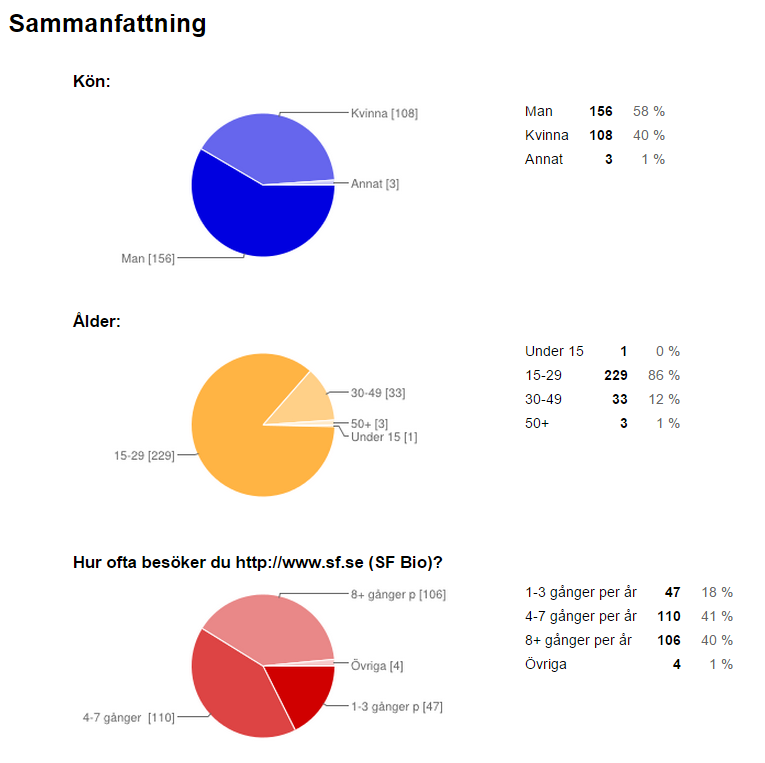
\includegraphics[scale=0.8]{shart1.PNG} 
\caption{Ny design för menyn av valbara filmer}
\end{figure}

\begin{figure}[H]
\centering
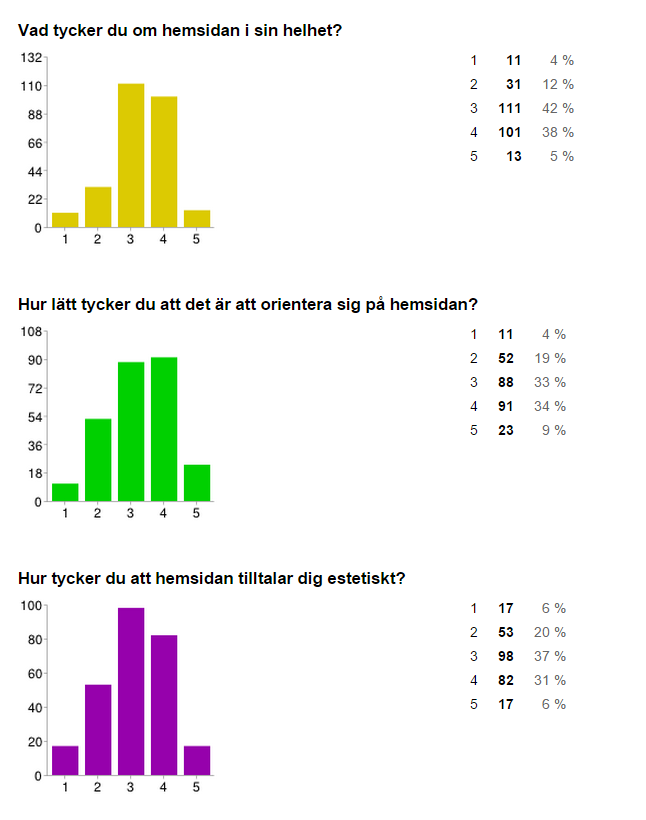
\includegraphics[scale=0.8]{shart2.PNG} 
\caption{Ny design för menyn av valbara filmer}
\end{figure}

\begin{figure}[H]
\centering
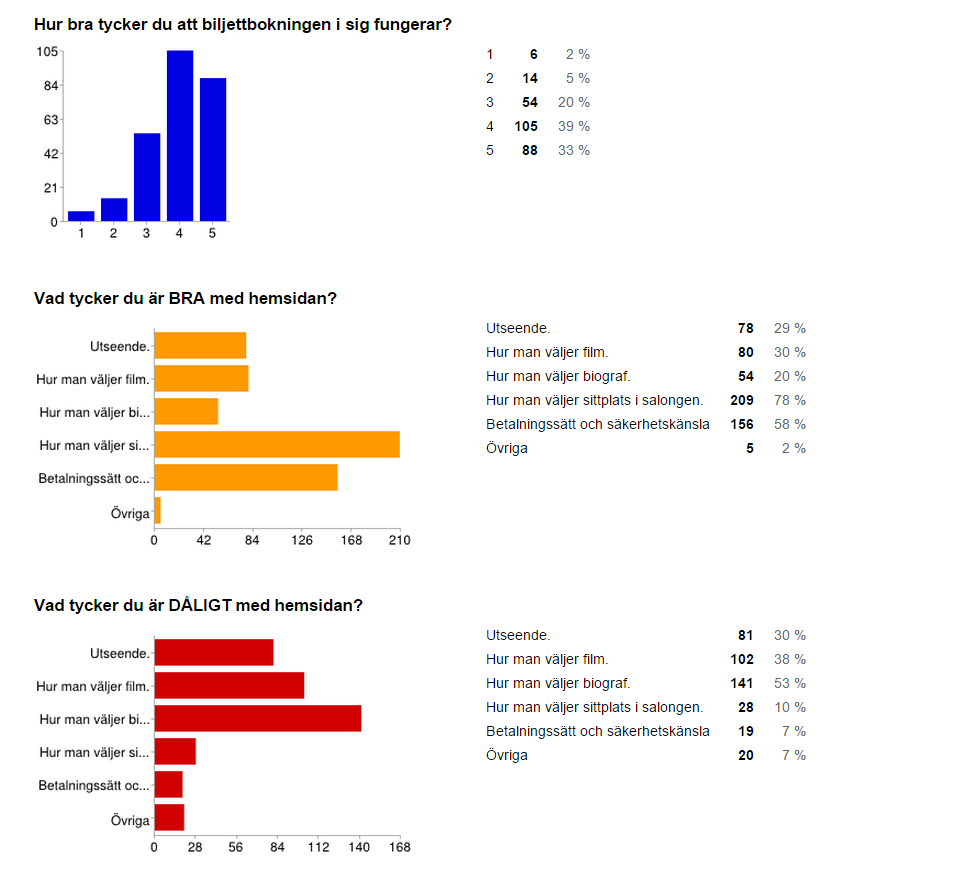
\includegraphics[scale=0.8]{shart3.PNG} 
\caption{Ny design för menyn av valbara filmer}
\end{figure}


\newpage
\section{Källor}

\begin{enumerate}[label={[\arabic*]}]
  \item SF Bio, 2012  \\
\url{http://www.sf.se/om-sf-bio/sf-bios-verksamhet/}\\{(Hämtad 2015-02-05)}

  \item Statistiska Centralbyrån, 2013\\
\url{http://www.scb.se/Statistik/_Publikationer/LE0108_2013A01_BR_IT01BR1401.pdf}\\{(Hämtad 2015-02-05)
} 
  
  \item Nielsen Norman Group. 2012 \url{http://www.nngroup.com/articles/thinking-aloud-the-1-usability-tool/}\\{(Hämtad 2015-02-05)}  
  
  \item Marcus Nystrand; Grafisk student på Beckmans Designhögskola. \\
2015, intervju den 4 Februari
  
  \item Sernheim, Åsa-Sara; magister i bildterapi, konstnär och formgivare.\\ 
2015, intervju den 4 Februari
  
  \item Lind, Thomas; doktorand Uppsala universitet\\
\url{http://katalog.uu.se/empinfo/?languageId=1&id=N10-1507}
\end{enumerate}


\end{document}